\section{Algoritmos de Reconhecimento}
\label{sec:algoritmos}
Existem diversos algoritmos de reconhecimento de caracter�sticas, entretanto
 nesse artigo os testes ser�o restritos aos algoritmos BRISK, FAST, FREAK, GFTT, MSER, ORB,
 STAR, SURF e SIFT por serem as t�cnicas mais utilizadas pelo meio de vis�o
 computacional no contexto de reconhecimento de caracter�sticas.
  Este cap�tulo se prop�e a dar uma vis�o geral dos algoritmos, pois o foco do presente trabalho est� na an�lise comparativa dos resultados obtidos no contexto
e n�o nas implementa��es, visto existir implementa��es conceituadas no OpenCV,
\emph{framework} utilizado, apresentado na Se��o \ref{sec:opencv}.

%\subsection{BRIEF - Binary Robust Independent Elementary Features}



 \subsection{FAST}


Segundo \cite{FAST}, � um m�todo de reconhecimento baseado em detec��o de
arestas originalmente desenvolvido por Edward Rosten e Tom Drummond. A maior
promessa do m�todo � a efici�ncia computacional O m�todo considera um c�rculo de dezesseis pixels ao redor da aresta considerada p. 
O detector original \cite{FusingPoints},\cite{VideoAnotation} classifica p como
uma aresta se existem n pixels cont�guos em um c�rculo que s�o mais brilhantes do que o pixel candidato de intensidade Ip mais
 um threshold t ou mais escuros do que Ip-t

 \begin{figure}[h!]
\centering
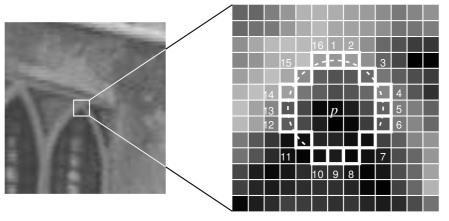
\includegraphics[scale=0.8]{images/fast01}
\caption{FAST}
\label{fig:fast01}
\end{figure}


Na imagem~\ref{fig:fast01} foi escolhido n=12. Um teste r�pido �
\begin{enumerate}
	\item Selecionar o ponto � testar primeiro as extremidades. no caso da imagem,
	escolhido o ponto p
	\item Comparar os pontos 1 e 9, e verifica-se se o ponto p tem intensidade
	com diferen�a de m�dulo t, ou seja os pontos 1 e 9 s�o mais claros ou mais escuros do que o ponto p pelo fator de t
	\item Avaliar se o ponto p continue sendo um candidato considerando os pontos 5
	e 13
	\item Analisar se p � uma aresta, sendo pelo menos 3 desses pontos devem ser
	mais brilhantes ou mais escuros do que p ent�o o teste pode ser feito nos demais pontos.
\end{enumerate}


 \subsection{BRISK - Binary Robust Invariant Scalable Keypoints}

Como descrito em \cite{BRISK}, ao contr�rio dos descritores vetoriais, como SURF
e SIFT, BRISK utiliza descritores no espa�o bin�rio o que para dispositivos com restri��o de recursos e poder computacional como dispositivos mobiles pode ser interessante.
Baseado no detector da t�cnica FAST, o processo consiste de tr�s partes.

\textbf{Amostragem de padr�es}

Retirando um padr�o de amostras ao redor do keypoint referentes a pontos espalhados em circulos conc�ntricos, que s�o usados para determinar se o ponto deve ou n�o ser selecionado como em um detector FAST.
As amostras s�o separadas em pares de dois subsets, curta dist�ncia e longa dist�ncia.

\textbf{Compensa��o de Orienta��o}
%REFAZER

Para atingir invari�ncia a rota��o, a dire��o de cada keypoint � determinada
tomando a soma dos gradientes locais calculados entre pares de longa dist�ncia e
os pares de curta dist�ncia s�o rotacionados baseados na orienta��o obtida.

\textbf{Compara��o de pares de amostragem}

 \begin{figure}[H]
\centering
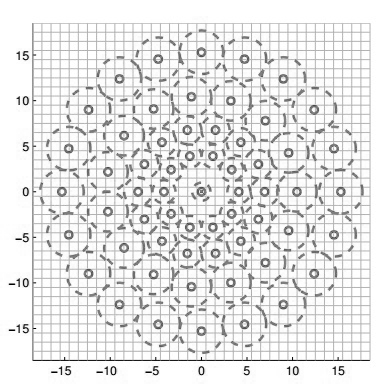
\includegraphics[scale=0.8]{images/brisk-descriptor}
\caption{Padr�o de amostras no BRISK}
\label{fig:briskdescriptor}
\end{figure}


Como mostrado na figura~\ref{fig:briskdescriptor}, BRISK possui um descritor
bin�rio de 512 bits que calcula a m�dia ponderada utilizando uma Gaussiana sobre um padr�o de pontos mais pr�ximos do ponto selecionado como mostrado na imagem~\ref{fig:briskdescriptor} no ponto (0,0). Ao longo do padr�o descrito, s�o aplicadas suaviza��es Gaussianas sendo que os c�rculos vermelhos representam o tamanho do desvio padr�o do filtro Gaussiano aplicado a cada ponto.
� baseado em compara��es entre pares de janelas de Gaussianas, resultando em 1 ou 0, dependendo de qual janela no par for maior.
Os pares ent�o s�o pr� selecionado no BRISK, criando descritores bin�rios que s�o posteriormente utilizados para casamento de padr�o, utilizando dist�ncias Hamming ao inv�s de Euclidianas.





 \subsection{FREAK - Fast Retina Keypoint}

FREAK � um descritor bin�rio, composto por tr�s etapas:

\textbf{Amostragem de padr�o}

FREAK prop�e uma abordagem biol�gica para o reconhecimento de caracter�sticas, emulando o funcionamento da retina para amostragem de padr�o, como demonstrado na imagem \ref{fig:freak-sampler} que � um padr�o circular com a diferen�a de ter maior densidade de pontos pr�ximo do centro. A densidade de pontos decresce exponencialmente.

\begin{figure}[H]
\centering
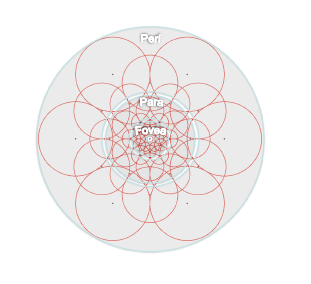
\includegraphics[scale=1.0]{images/freak-sampler}
\caption{Padr�o de amostradem do descritor FREAK}
\label{fig:freak-sampler}
\end{figure}


Cada amostra � suavizada com um kernel Gaussiano em que o raio do circulo ilustra o tamanho do desvio padr�o do kernel.
Como pode ser observado na figura~\ref{fig:freak-retina} o padr�o de amostragem corresponde com a distribui��o de receeptores na retina.

\begin{figure}[H]
\centering
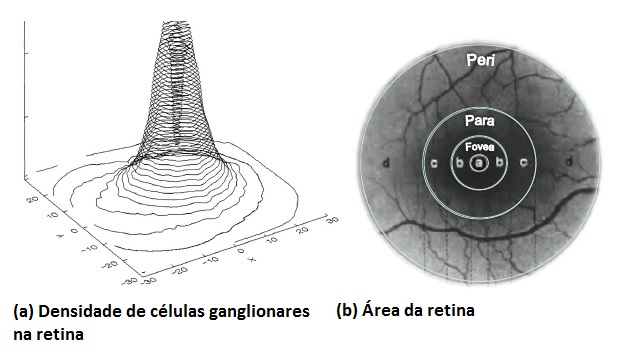
\includegraphics[scale=1.0]{images/freak-retina}
\caption{Distribui��o de receptores na retina}
\label{fig:freak-retina}
\end{figure}


\textbf{Compensa��o de Orienta��o}

Para estimar a rota��o dos keypoints, s�o somados os gradientes locais assim como no BRISK, entretanto ao inv�s de considerar os pontos de longa dist�ncia, s�o considerados 45 pontos como mostrado na figura~\ref{fig:freak-rotation}


\begin{figure}[H]
\centering
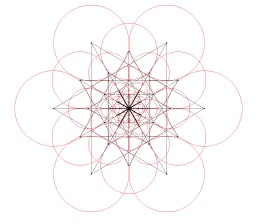
\includegraphics[scale=1.0]{images/freak-rotation}
\caption{Pares selecionados para calcular a orienta��o}
\label{fig:freak-rotation}
\end{figure}

Apesar de ter menos precis�o para recuperar informa��es de reota��o, como o n�mero de pontos � bem menor do que BRISK a quantidade de mem�ria armazenada � em geral mais do que 5 vezes menor.



\textbf{Compara��o de pares de amostragem}

Os pares de pontos s�o selecionados considerando a densidade maior no centro, como podemos observar na figura~\ref{fig:freak-retina} (a). Os pares come�am a ser comparados pelas extremidades e para dentro do centro, dessa forma otimizamos o reconhecimento pois com menos pontos podemos descartar casos em que a dist�ncia estiverem maiores do que um threshold, caso contr�rio prosseguimos para os outros 128 bits do descritor.



 \subsection{GFTT}
\label{sec:gftt}
 \subsection{MSER - \emph{Maximal Stable Extremal Regions}}

O detector MSER � composto por regi�es de todos os pixels conectados
considerando um \emph{threshold}. Em outras palavras, as regi�es selecionadas
s�o padr�es que n�o mudam e que a binariza��o local � est�vel ao longo de uma
faixa de \emph{thresholds}. Podemos fazer uma
analogia com o processo de forma��o de po�as de �gua para compreendermos como
s�o formadas as regi�es MSER, que s�o descritas em imagens em tons de cinza
representados pela fun��o $I: \Omega \rightarrow [0\ldots255] $ em que $\Omega =
[1 \ldots W]\times[1 \ldots H] $. O m�todo garante a localiza��o de objetos que
est�o mais pr�ximos de nossa realidade como pode ser observada na
Figura~\ref{fig:mserregion} \cite{MSER}.

 \begin{figure}[H]
\centering
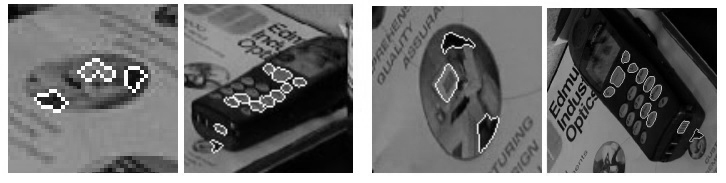
\includegraphics[scale=0.5]{images/mserregion}
\caption{Regi�es MSER. Fonte \cite{MSER}}
\label{fig:mserregion}
\end{figure}

Selecionado um \emph{threshold} de intensidades, a Figura � dividida em dois
grupos, P(pretos) e B(brancos). � observada que a quantidade de regi�es varia
dependendo do \emph{threshold} aplicado, de 0 a 255.
A �rea de cada componente conectado � ent�o armazenada como uma fun��o. Dentre
as regi�es, as mais est�veis s�o selecionadas analisando as fun��es para as quais
cada regi�o em potencial mantem seu estado com a mesma fun��o independente da
varia��o de \emph{threshold}. As regi�es ``m�ximamente est�veis'' s�o chamadas
regi�es MSER, que mudaram apenas em tamanho variando-se pelo menos alguns n�veis
de \emph{threshold}.




 \subsection{ORB - Oriented Fast and Rotated Brief}
\label{sec:orb}

%REFAZER
Como citado em \cite{ORB}, � uma combina��o de FAST e BRIEF.
 Para extrair \emph{keypoints}, modifica o detector do FAST construindo uma 
 piramide de escalas das imagems. Em cada escala \emph{keypoints} s�o
 detectados e a dist�ncia de Harris aplicada para selecion�-los, sendo somente
 os N melhores pontos selecionados de acordo com um \emph{threshold}.
Para obter invari�ncia � rota��o, momentos de primeira ordem s�o utilizados
 para calcular a orienta��o local atrav�s de um centr�ide que referencia a
  m�dia da magnitude dos pixels em um trecho local.
Posteriormente s�o calculados os descritores BRIEF nos trechos rotacionados
 e armazenadas as informa��es em um descritor ORB.




 \subsection{SIFT - Scale-Invariant Feature Transform}

M�todo baseado em detec��o de arestas que tem como proposta garantir a
invariancia a varia��o de escala. Um problema que nos m�todos de reconhecimento
de arestas se n�o tratado pode causar diminui��o na robustes do algoritmo. 
A figura~\ref{fig:sift01} ilustra bem o efeito que a mudan�a de escala pode
fazer.

\begin{figure}[h!]
\centering
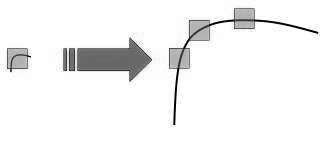
\includegraphics[scale=1.0]{images/SIFT01}
\caption{SIFT}
\label{fig:sift01}
\end{figure}

Em 2004, D.Lowe, descreveu o algoritmo Scale Invariant Feature Tranform no seu paper Distinctive Image
 Features from Scale-Invariant Keypoints[15] como extrair keypoints e computar os descritores.
8.10.2.1. Scale-space Extrema Detection
Observando a imagem~\ref{fig:sift01} � poss�vel notar que n�o podemos utilizar a
mesma janela de inspe��o independente da escala do objeto, para objetos maiores
temos que utilizar janelas maiores. Nesse contexto, o filtro scale-space �
utilizado e s�o calculados Laplacianos de Gaucianos com diversos valores de
$\sigma$.
  Os LoG funcionam como blob detectors que detectam
 blobs em v�rias escalas com a varia��o de $\sigma$.

Utilizar Laplacianos de Gaucianos � uma abordagem custosa computacionalmente,
como uma forma de aproxima��o s�o utilizados diferen�as de Gaucianas.


\begin{figure}[h!]
\centering
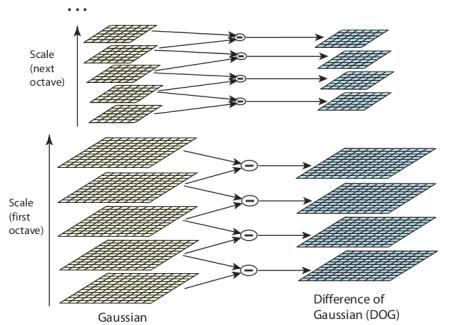
\includegraphics[scale=1.0]{images/DoG}
\caption{Difference of Gaussian}
\label{fig:dog01}
\end{figure}

Uma vez que as diferen�as de gaucianas s�o calculadas, � necess�rio procurar por
m�ximos entre espa�o e escalas diferentes. Por exemplo como mostrado na
figure~\ref{fig:dog02}, um pixel na imagem � comparado com seus 8 vizinhos e com
n�veis de escala pr�ximos e anteriores.
O que representa que o keypoint encontrado � melhor representado naquela escala.

\begin{figure}[h!]
\centering
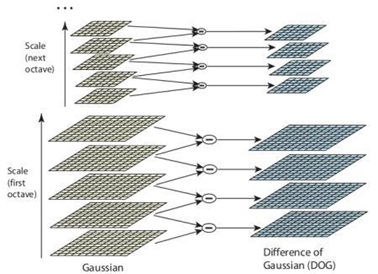
\includegraphics[scale=1.0]{images/DoG_escala}
\caption{Difference of Gaussian}
\label{fig:dog02}
\end{figure}



\subsubsection{Keypoint Localization}
Uma vez que keypoints potenciais s�o localizados � importante selecionar pontos de interesse com contraste alto.
A localiza��o dos pontos � refinada utilizando uma expans�o de Taylor  e se as intensidades dos m�ximos forem 
menores do que um threshold s�o rejeitados.
Uma caracter�stica do DoG � a alta resposta a arestas gerando falsos positivos. Portanto � necess�rio eliminar 
algumas arestas identificadas erroneamente.
\subsubsection{Orientation Assignment}
TODO
\subsubsection{Keypoint Descriptor}
TODO
\subsubsection{Keypoint Matching}
O casamento entre dois pontos � feito identificando pontos pr�ximos. Entretando em algumas citua��es existem
 pontos muito pr�ximos que podem ser causados por ruidos na detec��o de pontos de interesse, nesse caso � calculada
  uma raz�o de dist�ncia entre o ponto de interesse com o mais pr�ximo, e com o segundo mais pr�ximo, se a raz�o for
   maior do que 80 s�o rejeitados. Tal abordagem elimina cerca de 90 de falsos positivos e 5 de pontos corretos.




 \subsection{SURF - Speeded Up Robust Feature}

Segundo \cite{SURF} em compara��o com o algoritmo SIFT que aproxima Laplacianas
de Gaucinas por Diferencas de Gaucianas(DoG), SURF aproxima LoG de Box-type Filter e n�o �
utilizado nenhum tipo de suaviza��o entre escalas , o que garante mais agilidade
nos resultados porque a convolu��o com box filters s�o muito mais r�pidos com o uso de
 integral images e pode ser paralelizado

\begin{figure}[h!]
\centering
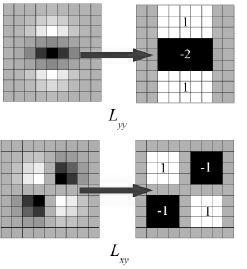
\includegraphics[scale=1.0]{images/SURF01}
\caption{Box Filtering}
\label{fig:surf01}
\end{figure}

Em geral SURF se apresenta cinco vezes mais r�pido do que DoG.
 \subsection{STAR}

Derivado de CenSurR(\emph{Center Surround Extrema}), STAR\cite{STAR}, assim como
SURF citado na Se��o~\ref{sec:surf} � baseado em \emph{box filters}. Entretanto,
enquanto DoB n�o � invariante � rota��o, � introduzido o filtro
\emph{center surroung} que s�o bi-level. A Figura~\ref{fig:bilevelfilter} mostra
o padr�o do filtro bi-level em v�rios n�veis, sendo o quanto mais circular, mais
preciso, entretanto tamb�m mais dif�cil de se calcular.
 
\begin{figure}[H]
\centering
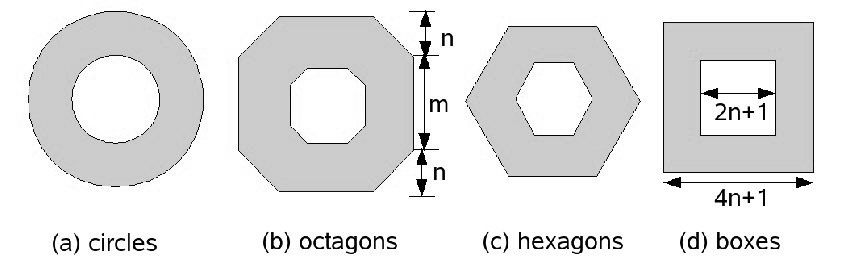
\includegraphics[scale=0.4]{images/bilevelfilter}
\caption{Filtro bi-level aplicado � formas de n lados. Fonte \cite{STAR}}
\label{fig:bilevelfilter}
\end{figure}


O detector de caracter�sticas de STAR em contrapartida � proposta do CenSurE,
usa um filtro composto de dois quadrados rotacionados. A resposta do filtro � calculada para sete escalas em cada pixel
da imagem. Em contraste com SIFT e SURF, o tamanho da amostra � constante em
cada escala e tende � resolu��o total em cada escala.
Um passo de p�s processamento � realizado para suprimir os n�o m�ximos e as
linhas.
Caracter�sticas que est�o ao longo de linhas s�o detectador devido � matriz de
gradientes, como apresentado na equa��o~\ref{eq:gftt}.


